\section{Estudo da Concavidade}

\subsection{Concavidade}
\begin{frame}
  \frametitle{Estudo da Concavidade}
  \begin{theorem}
    Se $f$ é uma função diferenciável em um intervalo aberto $I$, então o gráfico de $f$ é:
    \begin{enumerate}
      \item Côncavo para \textbf{cima} em $I$ se $f^{\prime}$ é \textbf{crescente} em $I$.
      \item Côncavo para \textbf{baixo} em $I$ se $f^{\prime}$ é \textbf{decrescente} em $I$.
    \end{enumerate}
  \end{theorem}
  \begin{columns}[onlytextwidth]
    \begin{column}< 2- >{0.49\textwidth}
      \textbf{Note que:} podemos estudar a monotonia de $f^{\prime}$ através de sua derivada! Se $f^{\prime}$ for diferenciável para $x\in I$, isto é, existir $f^{\prime\prime}(x)$, então:
      \begin{itemize}
        \item Pode ser verificado que $f^{\prime}$ é \textbf{crescente} em $I$ ao checar $f^{\prime\prime}(x) > 0$
        \item Semelhantemente, pode ser verificado que $f^{\prime}$ é \textbf{decrescente} em $I$ ao checar $f^{\prime\prime}(x) < 0$
      \end{itemize}
    \end{column}
    \begin{column}<3>{0.5\textwidth}\vspace{-0.5cm}
      \begin{block}{Teste da Segunda Derivada}
        Se $f$ é duas vezes diferenciável em um intervalo aberto $I$, então o gráfico de $f$ é:
        \begin{enumerate}
          \item Côncavo para \textbf{cima} em $I$ se $f^{\prime\prime}(x) > 0$ para todo $x$ em $I$.
          \item Côncavo para \textbf{baixo} em $I$ se $f^{\prime\prime}(x) < 0$ para todo $x$ em $I$.
        \end{enumerate}
      \end{block}
    \end{column}
  \end{columns}
\end{frame}

\begin{frame}
  \vspace{0.75cm}
  \begin{figure}
    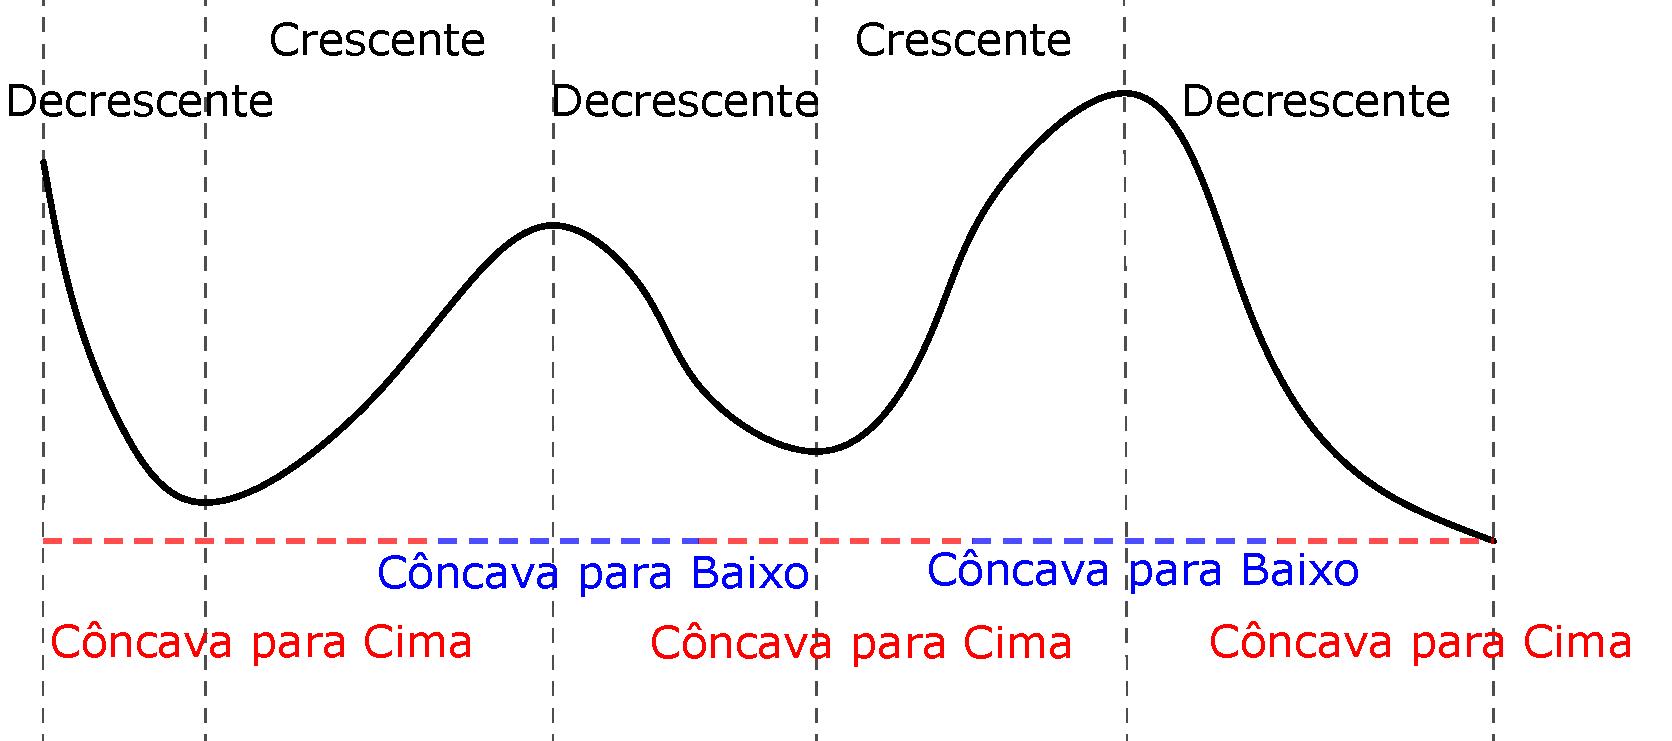
\includegraphics[width=\textwidth]{figuras/figura1.pdf}
  \end{figure}
\end{frame}

\begin{frame}
  \begin{figure}
    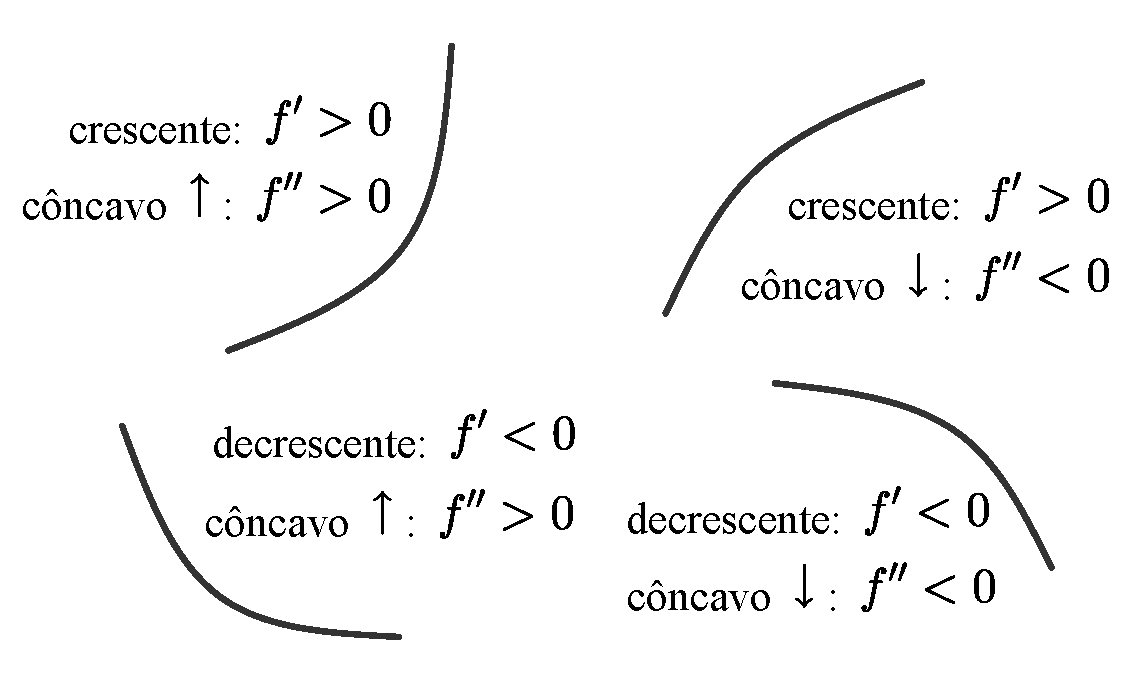
\includegraphics[width=0.9\textwidth]{figuras/figura2.pdf}
  \end{figure}
\end{frame}

\subsection{Exemplo 1}
\begin{frame}
  \begin{columns}[onlytextwidth]
    \begin{column}{0.5\textwidth}\vspace{-0.85cm}
      \begin{block}{Exemplo 1}
        Faça o estudo da concavidade da função $f(x) = x^{3} - 6x^{2} + 8x + 5$.
      \end{block}
    \end{column}
    \begin{column}{0.5\textwidth}\vspace{-0.75cm}
    \end{column}
  \end{columns}
\end{frame}

\section{Pontos de Inflexão}

\begin{frame}
  \begin{definition}
    Um  ponto $(x_{0},f(x_{0}))$ do gráfico de uma função $f$ é chamado de \textbf{ponto de inflexão} se forem verificadas as duas condições:
    \begin{enumerate}
      \item $f$ é \emph{contínua} em $c$
      \item Existe um intervalo $]a,\,b[$ contendo $x_{0}$ tal que $f$ tem seu gráfico \emph{côncavo para cima} em $]a,x_{0}[$ e \emph{côncavo para baixo} em $]x_{0},b[$, ou \emph{vice-versa}
    \end{enumerate}
  \end{definition}
  \begin{figure}
    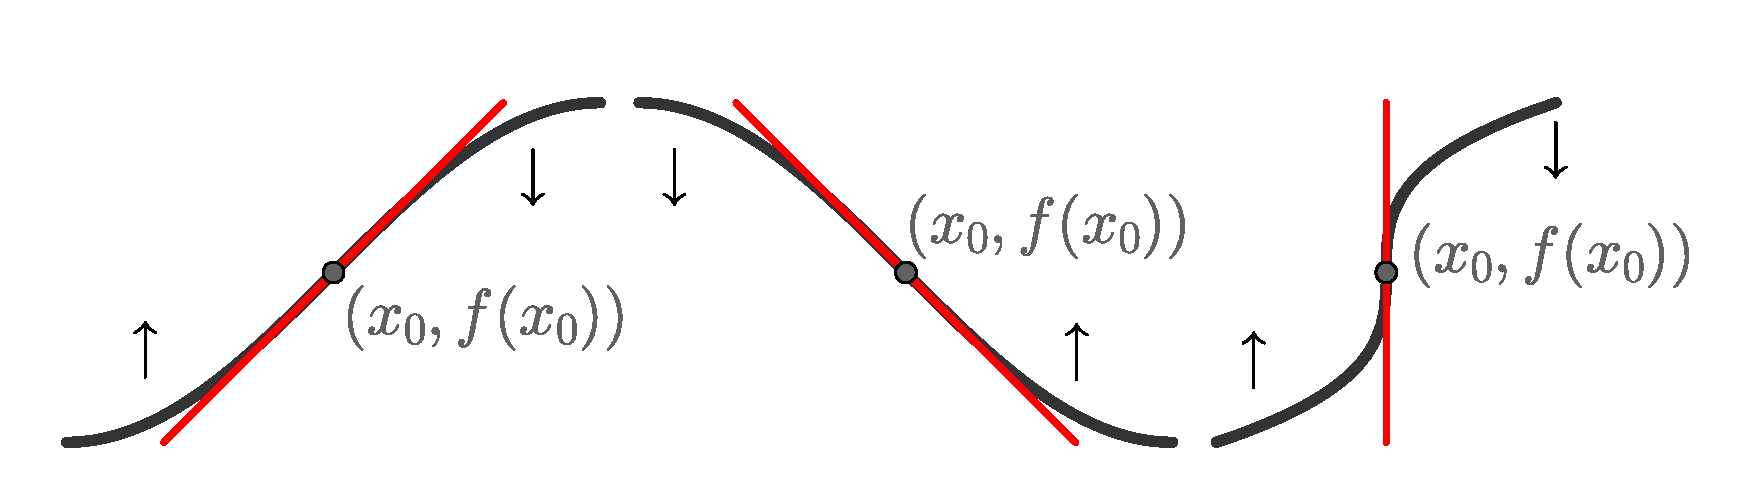
\includegraphics[width=0.9\textwidth]{figuras/figura3.pdf}
  \end{figure}
\end{frame}

\begin{frame}
  \begin{theorem}[Teste da 2ª derivada para a determinação de extremos de uma função]
    Seja $f$ função \emph{duas vezes} diferenciável em um intervalo aberto $I$ contendo $x_{0}$ tal que \mbox{$f^{\prime}(x_{0}) = 0$}.
    \begin{enumerate}
      \item Se $f^{\prime\prime}(x_{0}) < 0$, então $f$ tem um \textbf{máximo local} em $x_{0}$.
      \item Se $f^{\prime\prime}(x_{0}) > 0$, então $f$ tem um \textbf{mínimo local} em $x_{0}$.
    \end{enumerate}
  \end{theorem}
  \begin{columns}[onlytextwidth]
    \begin{column}{0.45\textwidth}\vspace{-0.9cm}
      \begin{figure}
        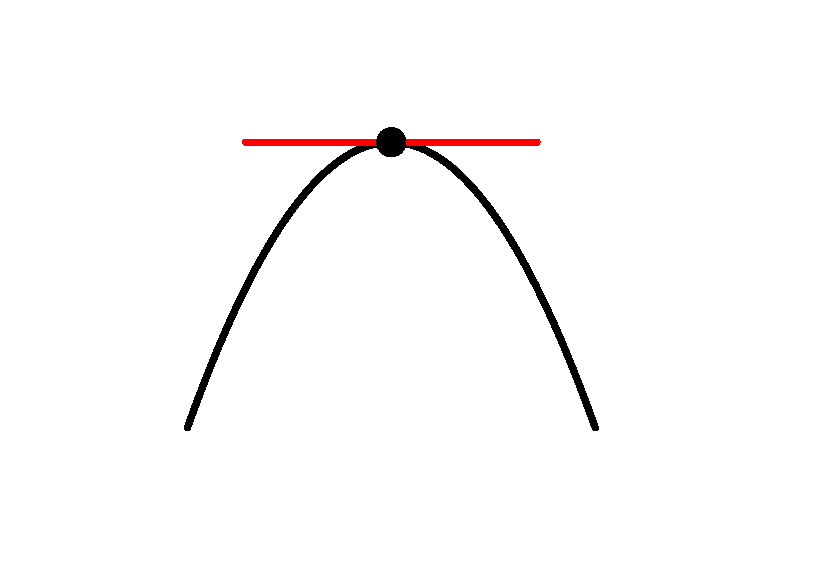
\includegraphics[width=\textwidth]{figuras/fig6.pdf}
      \end{figure}
    \end{column}
    \begin{column}{0.45\textwidth}\vspace{-0.9cm}
      \begin{figure}
        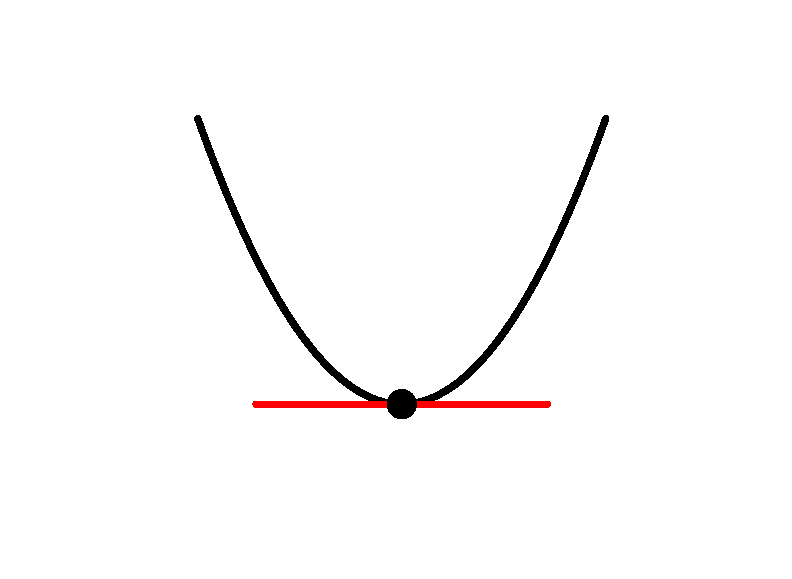
\includegraphics[width=\textwidth]{figuras/fig7.pdf}
      \end{figure}
    \end{column}
  \end{columns}
\end{frame}

\subsection{Exemplo 2}
\begin{frame}
  \begin{columns}[onlytextwidth]
    \begin{column}{0.65\textwidth}\vspace{-0.85cm}
      \begin{block}{Exemplo 2}
        Determine os extremos locais das seguintes funções:
      \end{block}
      \begin{enumerate}
        \item<only@+> $f(x) = x^{2} + 2x - 3$
        \item<only@+> $g(x) = x + \dfrac{1}{x}$
      \end{enumerate}
    \end{column}
    \begin{column}{0.35\textwidth}\vspace{-0.75cm}
    \end{column}
  \end{columns}
\end{frame}

\section{Construção de Gráficos}

\begin{frame}
  \frametitle{Construção de Gráficos}
  O esboço do gráfico de uma função pode ser obtido a partir do seguinte roteiro:
  \begin{columns}[onlytextwidth]
    \begin{column}{0.48\textwidth}
      \begin{enumerate}
        \item Identificar o domínio;
        \item Determinar os pontos de interseção com os eixos cartesianos (se possível);
        \item Verificar a existência de assíntotas;
        \item Fazer o estudo da monotonia;
        \item Verificar a existência de pontos extremos (Pontos críticos);
      \end{enumerate}
    \end{column}
    \begin{column}{0.48\textwidth}
      \begin{enumerate}\setcounter{enumi}{5}
        \item Fazer o estudo da concavidade;
        \item Verificar a existência de pontos de inflexão;
        \item Localizar os pontos extremos e de inflexão no sistema cartesiano;
        \item Construir o esboço do gráfico.
      \end{enumerate}
    \end{column}
  \end{columns}
\end{frame}

\begin{frame}
  \begin{figure}
    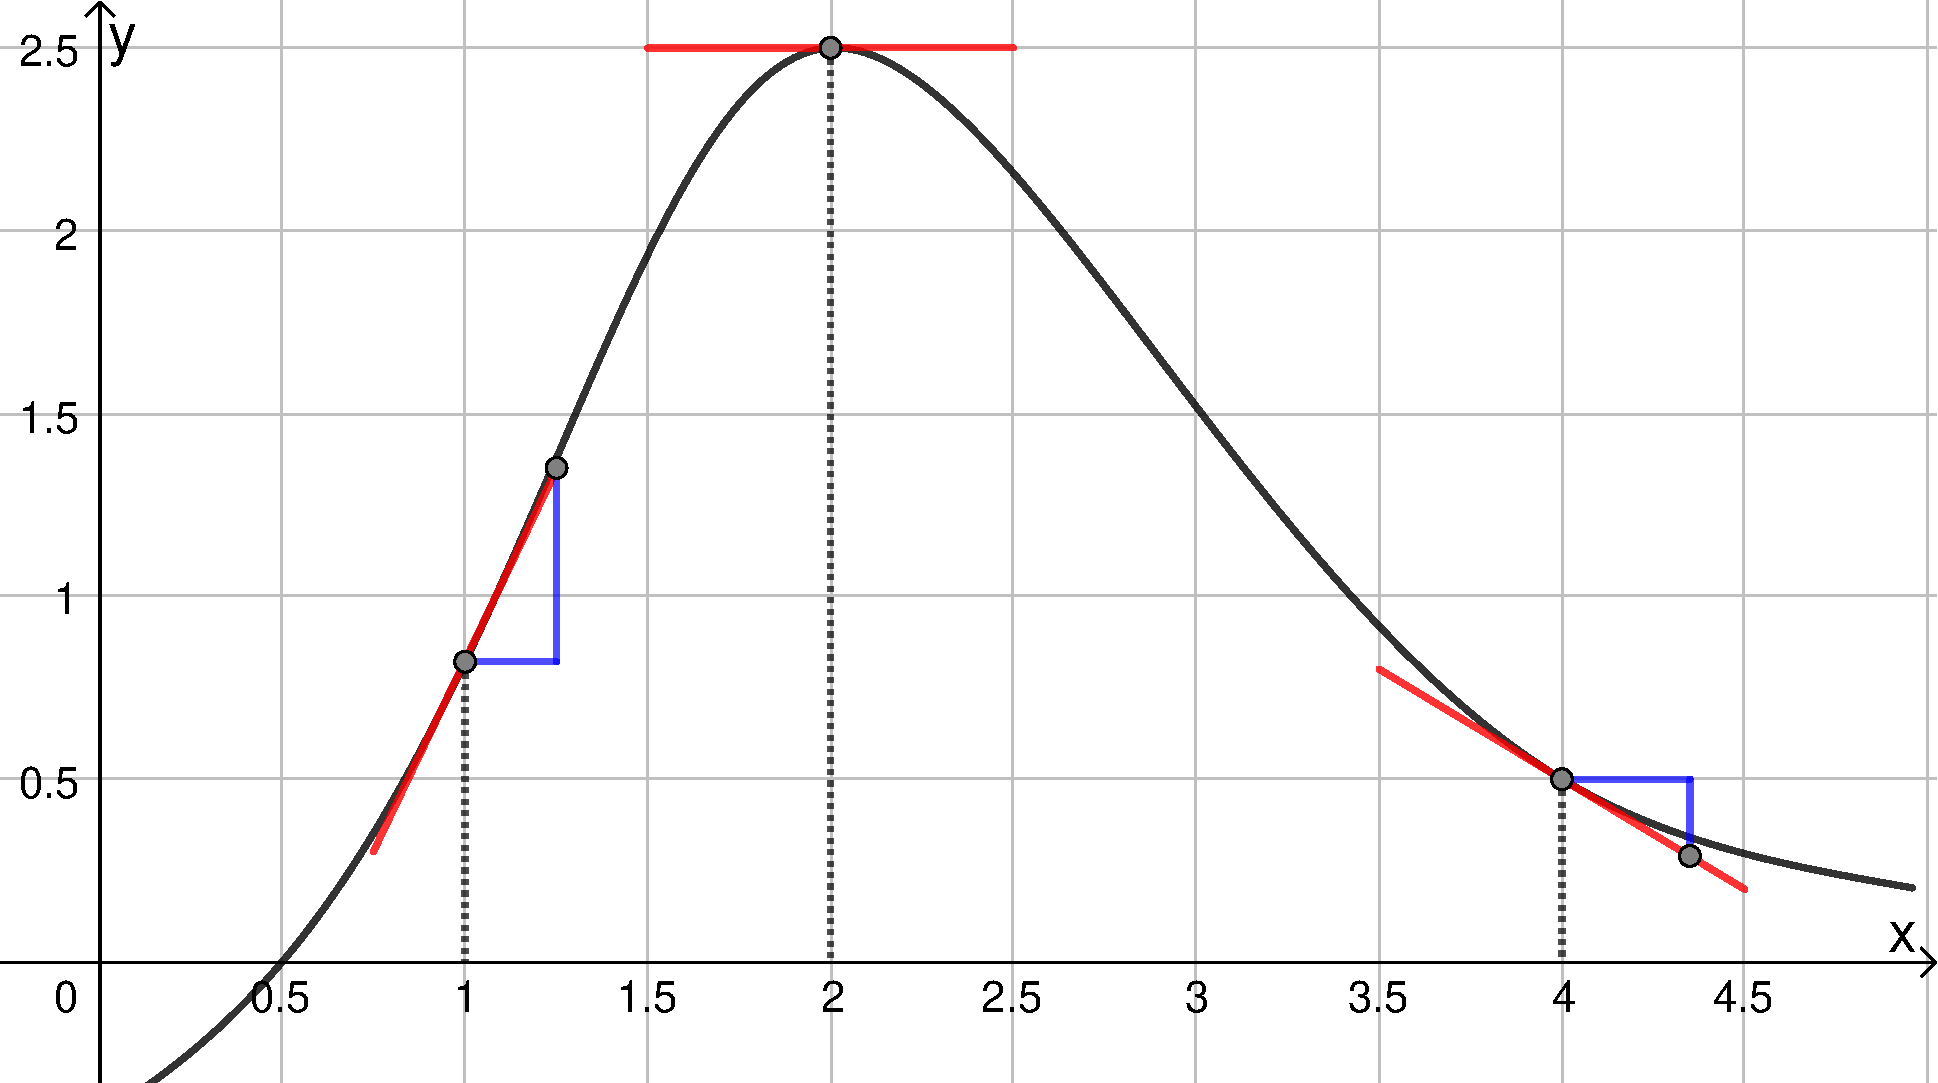
\includegraphics[width=0.95\textwidth]{figuras/figura4.pdf}
  \end{figure}
\end{frame}

\subsection{Exemplo 3}
\begin{frame}
  \begin{columns}[onlytextwidth]
    \begin{column}{0.45\textwidth}\vspace{-0.85cm}
      \begin{block}{Exemplo 3}
        Sobre a função $f(x) = x^{4} - 4x^{3} + 10$:
      \end{block}
      \begin{enumerate}
        \item<only@+> Estude a sua monotonia;
        \item<only@+> Determine os pontos extremos;
        \item<only@+> Estude a concavidade;
        \item<only@+> Determine pontos de inflexão;
        \item<only@+-> Esboce o gráfico de $f$.
      \end{enumerate}
    \end{column}
    \begin{column}{0.55\textwidth}\vspace{-0.95cm}
      \begin{figure}
        \includegraphics<5>[width=0.9\textwidth]{figuras/figura5-2.pdf}
        \includegraphics<6>[width=0.9\textwidth]{figuras/figura5.pdf}
      \end{figure}
    \end{column}
  \end{columns}
\end{frame}

\subsection{Exemplo 4}
\begin{frame}
  \begin{columns}[onlytextwidth]
    \begin{column}{0.45\textwidth}\vspace{-0.85cm}
      \begin{block}{Exemplo 4}
        Sobre a função $f(x) = \dfrac{x^{2}}{x^{2} - 4}$:
      \end{block}
      \begin{enumerate}
        \item<only@+> Determine o domínio de $f$;
        \item<only@+> Determine os pontos de interseção com os eixos;
        \item<only@+> Determine as assíntotas de $f$;
        \item<only@+> Estude a sua monotonia;
        \item<only@+> Determine os pontos extremos;
        \item<only@+> Estude a concavidade;
        \item<only@+> Determine pontos de inflexão;
        \item<only@+-> Esboce o gráfico de $f$.
      \end{enumerate}
    \end{column}
    \begin{column}{0.55\textwidth}\vspace{-0.85cm}
      \begin{figure}
        \includegraphics<8>[width=0.8\textwidth]{figuras/figura6-2.pdf}
        \includegraphics<9>[width=0.8\textwidth]{figuras/figura6.pdf}
      \end{figure}
    \end{column}
  \end{columns}
\end{frame}